\begin{figure*}[t!]
	\begin{center}
		\begin{tabular}{c}
		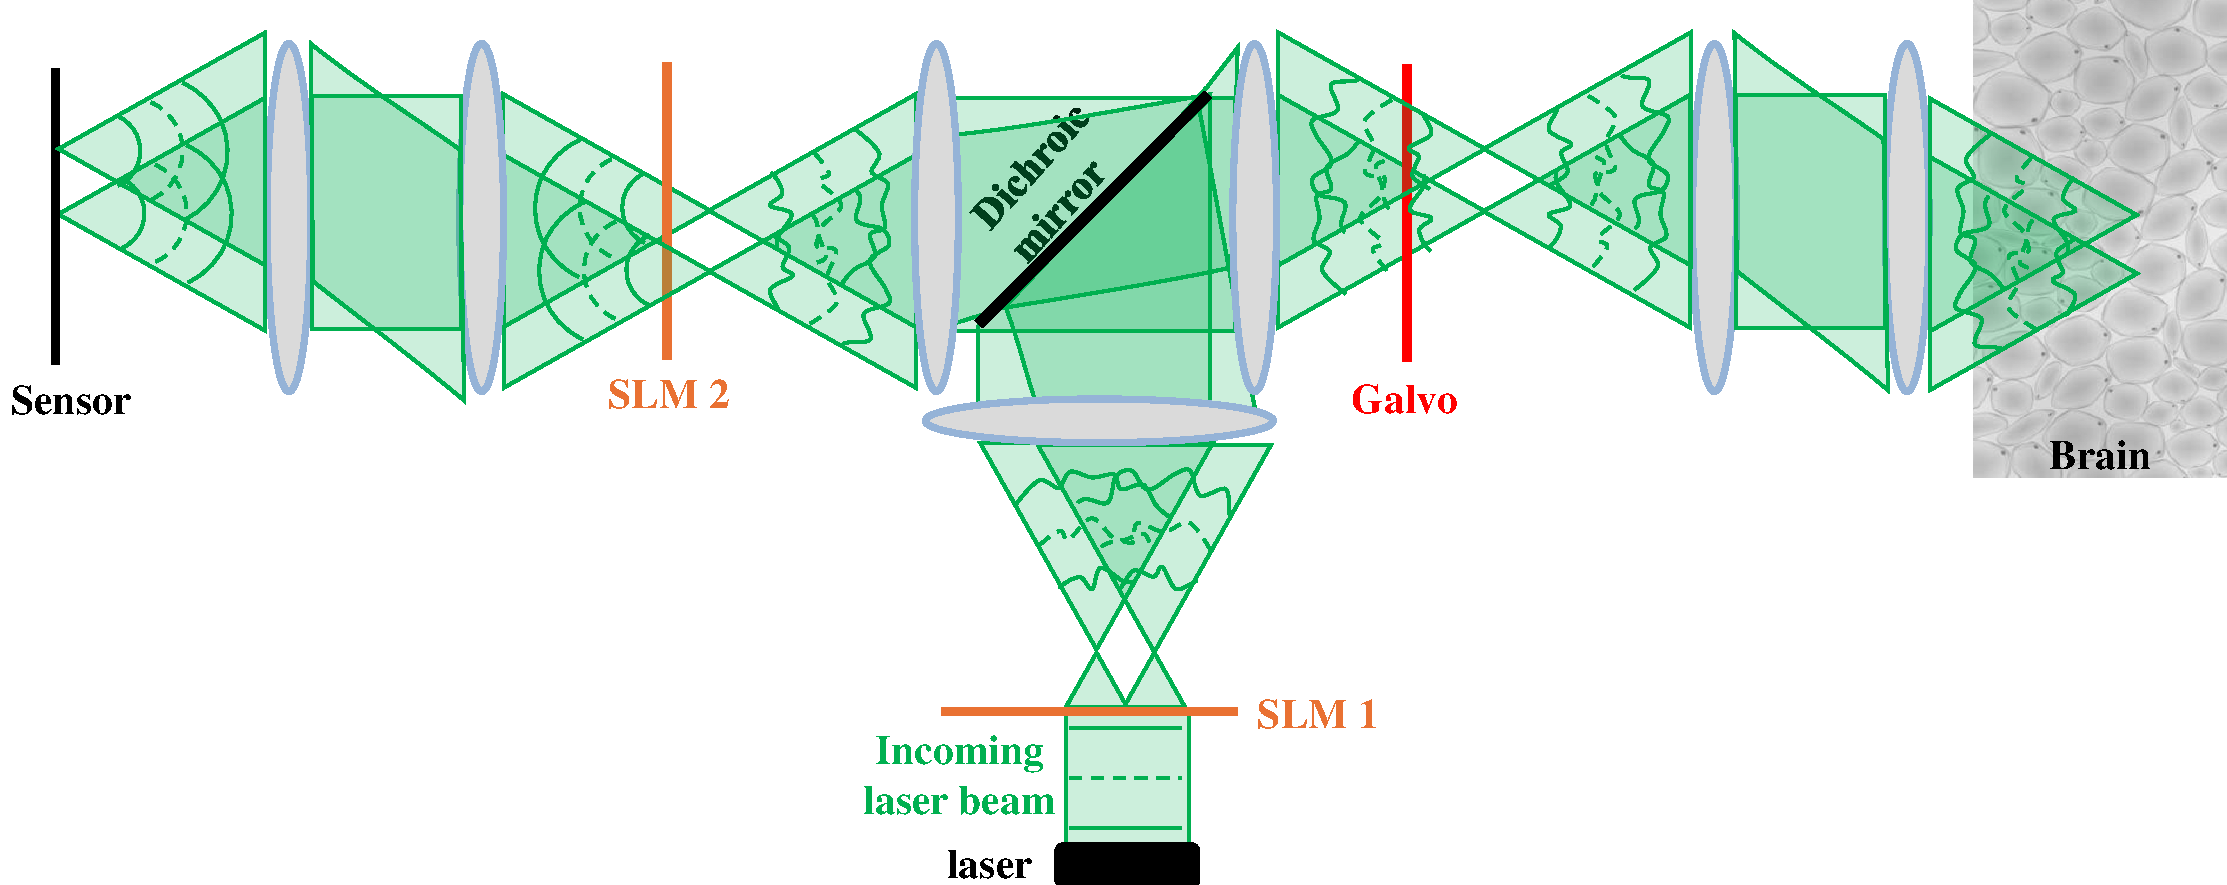
\includegraphics[width= 0.8\textwidth]{figs/system/twoP.pdf}
		%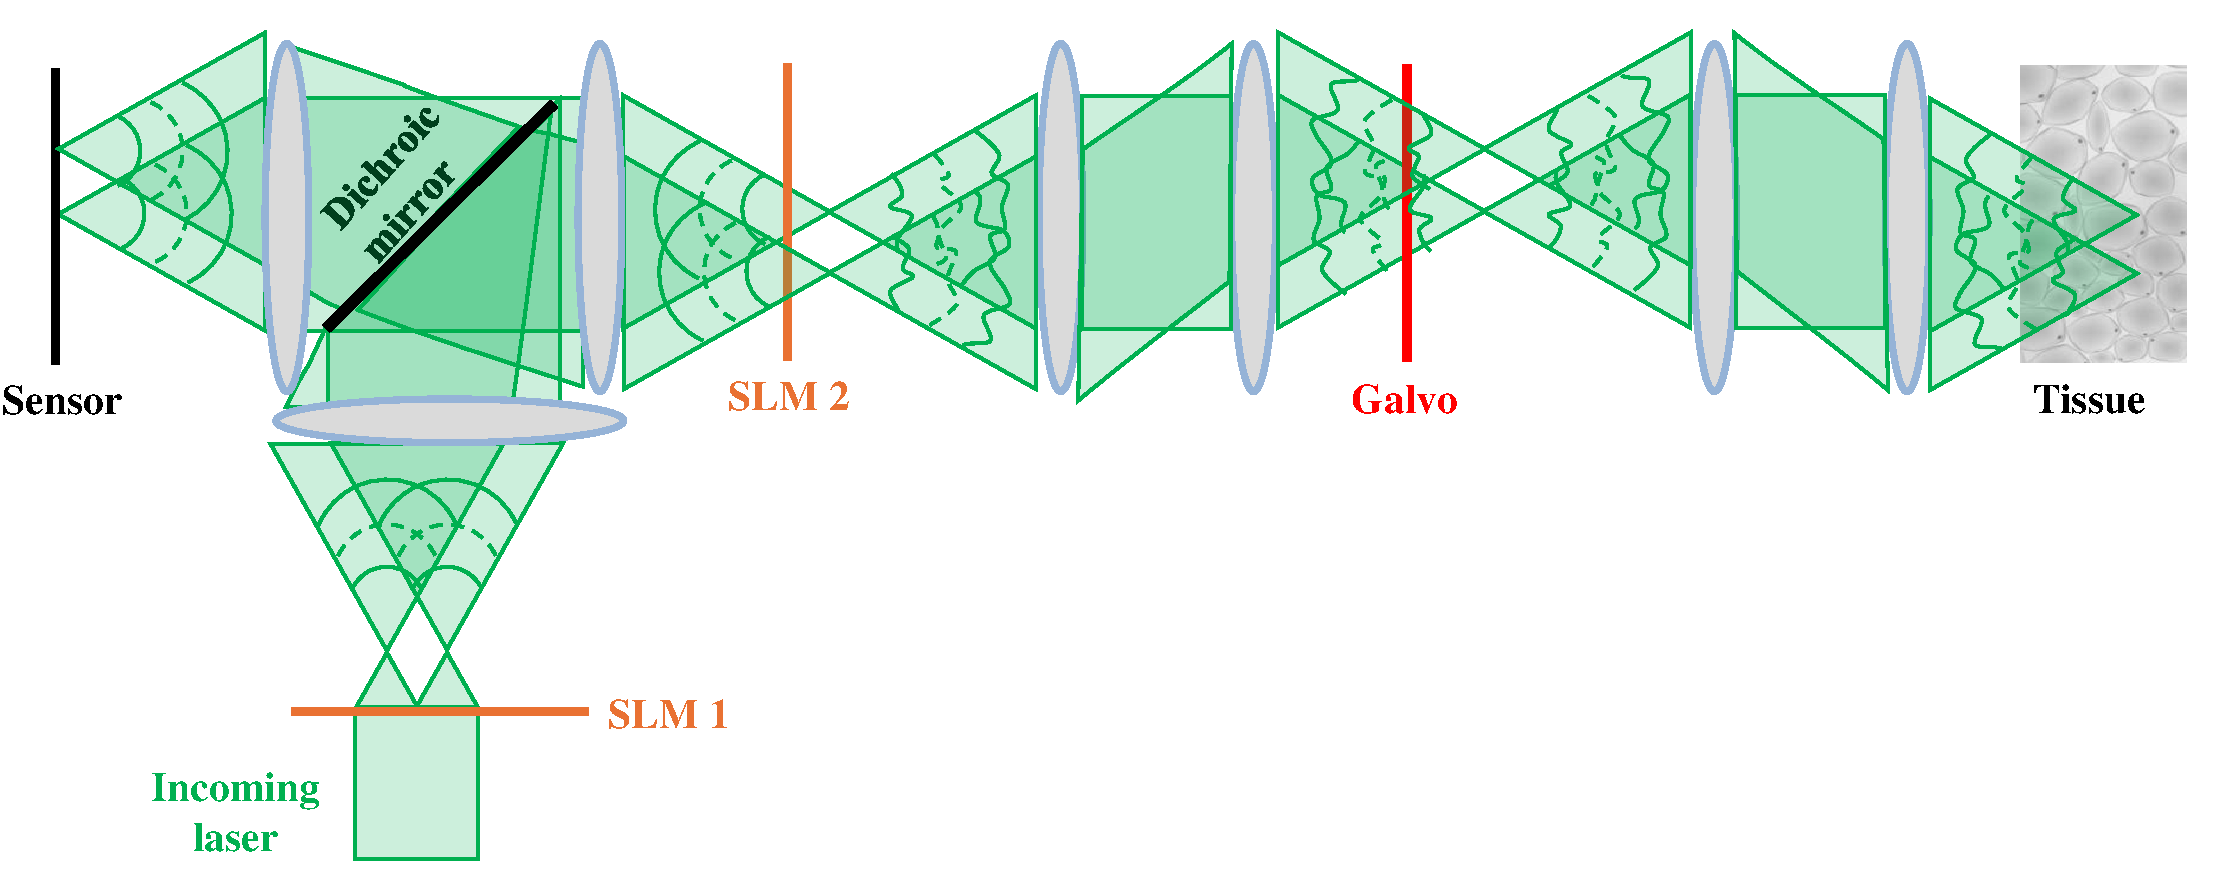
\includegraphics[width= 0.48\textwidth]{figs/system/oneP.pdf}\\
		%(a) Two photon&(b) One photon
		\end{tabular}
	\end{center}
	\caption{{\bf{Wavefront-shaping setup:}} SLM1 generates a hologram directing excitation light to different target neurons, this hologram can also reshape the light to account for tissue aberration. The emitted light is collected via the same objective but directed toward a sensor via a dichroic mirror. The aberration of these wavefronts are corrected at SLM2. The figure illustrates two target neurons at different positions, which are mapped using different SLM pixels. The setup also includes a galvo, which is aimed to scan a diffraction limited illumination point over the neuron area.  } 
%	\caption{{\bf{Wavefront-shaping setup:}}(a) 2P setup: SLM1 generates a hologram directing excitation light to different target neurons, this hologram can also reshape the light to account for tissue aberration. The emitted light is collected via the same objective but directed toward a sensor via a dichroic mirror. The aberration of these wavefronts are corrected at SLM2. The figure illustrates two target neurons at different positions, which are mapped using different SLM pixels. The setup also includes a galvo, which is aimed to scan a diffraction limited illumination point over the neuron area. (b) 1P setup: As the excitation and emission wavefront are similar, they require the same correction pattern, and thus are both modulated at SLM2. In this setup SLM1 is only used to generate two diffraction limited points at the positions of the target neurons.  } 
\label{fig:setup}
\end{figure*}

